\chapter{Approximations}
\graphicspath{{../gfx/chapter02/}{../plots/chapter02/}}

% TODO: in chapter 1: change V_2 -> V_0
% TODO: include a graph showing the broadening of peaks with temperature and
% hence how the singlet-triplet splitting gets washed out

To access larger systems we need to introduce approximations. Approximating
means to simplify. However, by carefully establishing successive approximations
and their limits, we also reduce the problem to its essential ingredients and
thus, hopefully, we gain a better understanding of the system. Our first
approximation is somewhat ad hoc and motivated by the very ideas underlying the
QCA approach. QCA relies on two electrons per cell (or, more generally, a fixed
number of charges per cell). Therefore we truncate the Hilbert space and keep
only states with two electrons in each cell. We omit the chemical potential
term, $\mu = 0$. This \emph{fixed charge} approximation obviously does not allow
for charge fluctuations and consequently cannot accommodate inter-cell hopping.
We justify the approximation by noting that, at least in principle, for any
given cell layout we can always tune the system parameters (especially the chemical
potential) so that we have two electrons per cell. Of course, in practice there
are very clear limits as to how much system parameters can be tuned and any QCA
cell layout considered within the \emph{fixed charge} approximation cannot
necessarily be readily implemented on a given real-world material system.

For the \emph{fixed charge} system, the state space scales as $N_s =
\binom{8}{2}^{N_c} = 28^{N_c}$ ($N_c$ is the number of cells). Again, we utilize
symmetries to make the Hamiltonian matrix block diagonal and as before the
largest block is the spin zero sector, of size $N_s^{\prime} = 16^{N_c}$. This
corresponds to a memory consumption of 512kB, 128MB, and 32GB for two, three and
four cell systems, respectively. That's doable. Five cells, however, remain
impossible. To illustrate how the approximation works
Fig.~\ref{fig:fixed_charge_approximation}(a) compares the density of states
(more correctly, the energy state histogram) of both the \emph{fixed charge}
and the exact \emph{grand canonical} system. The \emph{fixed charge}
approximation accurately reproduces the low-energy spectrum of the \emph{grand
canonical} model. This is not unexpected. As long as the QCA system is in the
right regime, the two-electrons-per-cell sector is lowest in energy. It is in
this limit, with the temperature additionally smaller than the energy gap to the
next higher charge sector, that the approximation is valid.
Fig.~\ref{fig:fixed_charge_approximation}(b) demonstrates the breakdown of the
approximation. Here we have plotted the particle number per cell over
temperature and as the temperature is increased and becomes comparable to the
energy gap, the \emph{fixed charge} and \emph{grand canonical} systems diverge.
%
\begin{figure}
  \center
  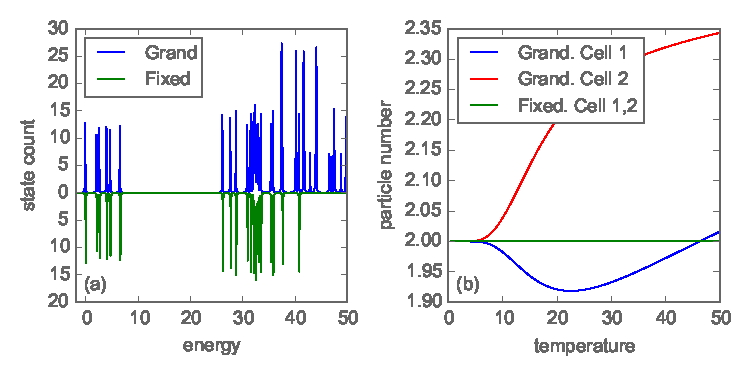
\includegraphics{fixed_charge_approximation}
  \caption{(a) Low-energy density of states of the exact \emph{grand canonical}
  and the approximative \emph{fixed charge} two cell QCA system. For small
  energies the curves agree perfectly (up to $E \lesssim 35$). (b) Particle
  number per cell over temperature for the same two cell system. The curves
  diverge for $T \gtrsim 5$.}
  \label{fig:fixed_charge_approximation}
\end{figure}
%

As evidenced by our semi-classical introduction at the beginning of this report,
the QCA approach does not consider particle spins. It solely relies on
charge-charge interactions. Therefore it is natural to the QCA approach to
neglect the spin degree of freedom as a next step. The 28 states per cell of the
\emph{fixed charge} model can be reorganized into four doubly occupied dots and
six bonds, four along the edges and two along the diagonals of the cell. Each
bond consists of two electrons and corresponds to four states, one spin singlet
and three spin triplets. By keeping only one state for each bond and omitting
the doubly occupied states we arrive at the \emph{bond} approximation. It has a
basis of six states per cell, the six bonds. As a consequence, the size of the
Hilbert space is $N_s = 6^{N_c}$ ($N_c$ the number of cells). Five and six cells
are doable, with memory requirements of 460MB and 16GB, respectively, whereas
seven cells are not (580GB). Note that for the \emph{bond} model there are no
symmetries that can be exploited. 

%
\begin{figure}
  \center
  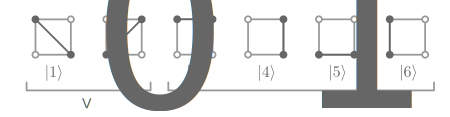
\includegraphics{bond}
  \caption{\ldots}
  \label{fig:bond}
\end{figure}
\begin{figure}
  \center
  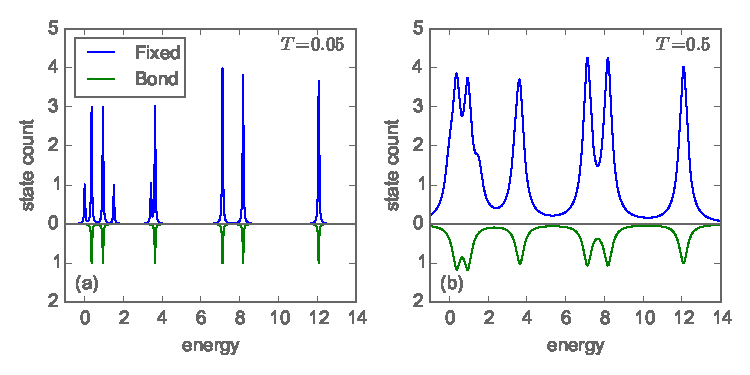
\includegraphics{bond_approximation1}
  \caption{Low-energy density of states of a one cell QCA system for both the
  \emph{fixed charge} and the \emph{bond} model. The \emph{bond} approximation
  does not reproduce the singlet-triplet splitting.}
  \label{fig:bond_approximation1}
\end{figure}
%
\begin{figure}
  \center
  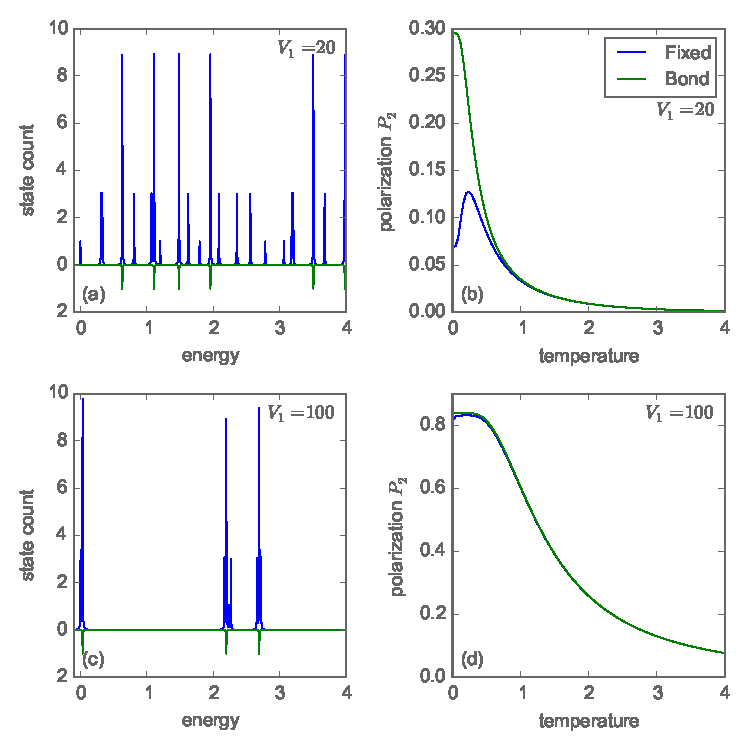
\includegraphics{bond_approximation2}
  \caption{The two cell \emph{fixed charge} and \emph{bond} systems at $V_1 =
  20$ and $V_1 = 100$. (a)(c) Low-energy density of states. (b)(d) Output
  polarization $P_2$ over temperature. For a small Coulomb repulsion the density
  of states curves look qualitatively very different (a) and the \emph{bond}
  approximation does not work very well (b). At a larger Coulomb repulsion the
  density of states curves look much more alike (c) and the \emph{bond}
  approximation works much better (d).}
  \label{fig:bond_approximation2}
\end{figure}
%
Apart from requiring sufficiently gapped out doubly occupied states, the
\emph{bond} approximation assumes that the bond singlet and triplet states are
energetically degenerate. But this is not quite correct. To understand
how the approximation works we look at the density of states (energy state
histogram, to be correct) of the single cell \emph{fixed charge} and \emph{bond}
systems, Fig.~\ref{fig:bond_approximation1}. Each \emph{bond} state maps to
three \emph{fixed charge} states---the triplet---and one ``close-by''
state---the singlet. Hence, singlet and triplet states are not equivalent, they
are split by an energy gap $\Delta E$. We speculate that, similar to the
antiferromagnetic Heisenberg coupling constant $J$ emerging in the low energy
limit of the Hubbard model (with $J \sim \frac{t^2}{U}$) \cite{Auerbach}, here,
virtual excitations to high energy doubly occupied states lower the energy of
the singlet state compared to the triplet state. Since the \emph{bond} model
ignores the singlet-triplet splitting it is important to understand how this gap
depends on various system parameters. To that end we picked out a few
selected singlet-triplet states from the spectrum in
Fig.~\ref{fig:bond_approximation1} as examples. Contrary to expectations, for
those states the gap $\Delta E$ did not change significantly with the on-site
Coulomb repulsion $U$, however, it did decrease with decreasing $b$, the
inter-cell spacing. Most importantly, for the nearest-neighbour Coulomb
potential, $V_1 = \frac{1}{a}$ ($a$ being the cell side length), we found
$\Delta E \sim \frac{1}{V_1^p}$. The exponent is $p \sim 3$ when the cell
``sees'' a biasing external potential (e.g.\ $P_0 = \pm 1$) and $p \sim 1$
otherwise (e.g.\ $P_0 = 0$). Even though our method is anything but rigorous and
the obtained results very likely not universally true, the findings should
nonetheless give a good enough idea of the principle trends. Quite generally,
the higher the overall Coulomb potential (large $V_1$, small $b$), the smaller
the singlet-triplet splitting and, conceivably, the more accurate the
\emph{bond} approximation.

We expect the approximation to work as long as the
singlet-triplet splitting is ``washed out,'' that is, as long as the temperature
is much bigger than the gap $\Delta E$. As a very, very rough estimate we come
up with $T \gg \frac{t^2}{V_1}$. Of course, we also need $T \ll U$ so that the
doubly occupied states are gapped out. Outside of this loosely defined regime,
the \emph{bond} model can and does go terribly wrong. Especially the ground
state is often qualitatively completely incorrect. Consider, for example,
Fig.~\ref{fig:bond_approximation2}(b) where we have plotted the output
polarization $P_2$ of a two cell system over temperature. For this system we set
the input polarization $P_0 = 1$, the Hubbard $U$ is practically infinite, the
inter-cell spacing is $b = 2 a$, and the nearest-neighbour Coulomb repulsion has
the value $V_1 = \frac{1}{a} = 20$ (in units of $t$, $t=1$). The two curves for
the \emph{fixed charge} and the \emph{bond} system disagree at low temperatures.
It is instructive to compare the density of states of the two systems,
Fig.~\ref{fig:bond_approximation2}(a): They look quite different, qualitatively.
In that light it is rather remarkable that the polarization curves actually
agree quite well at higher temperatures ($T > 1$). The \emph{bond} model only
reproduces the most populous energy states of the exact spectrum. Apparently,
that is enough to give (almost) correct results at high temperatures. The lower
the temperature, the more important become the few lowest lying energy states
which the \emph{bond} model misses. For a larger Coulomb repulsion, $V_1 = 100$,
the density of states curves look much more alike, even though the \emph{bond}
model obviously still does not resolve all the lines of the exact spectrum,
Fig.~\ref{fig:bond_approximation2}(c). Accordingly, the approximation works much
better as can be seen in Fig.~\ref{fig:bond_approximation2}(d). As a last
remark, note that for the two cell system each single \emph{bond} state
corresponds to $16$ ($4 \cdot 4$) \emph{fixed charge} states.

%
\begin{figure}
  \center
  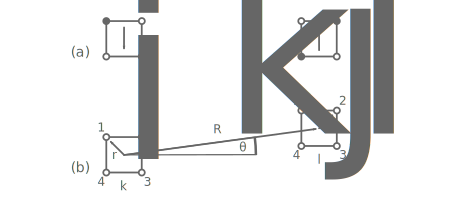
\includegraphics{ising}
  \caption{a) QCA cells $k$ and $l$. b) The two-states-per-cell approximation
  identifies each cell with a spin $\uparrow$ or $\downarrow$.}
  \label{fig:cells2}
\end{figure}
%
A linear array of QCA cells where each cell has a state of digital 0 or 1 is
reminiscent of a 1D spin $\frac{1}{2}$ chain. Indeed, if we reduce the basis to
only two states per cell (down from six states in the \emph{bond} picture) we
can map the QCA system to a transverse-field Ising model. This is an attractive
proposition: The smaller Hilbert space allows for larger system sizes with our
exact diagonalization method; much more importantly, the transverse-field Ising
model is amenable to sign-problem-free Stochastic series expansion (SSE) quantum
Monte Carlo schemes \cite{Sandvik2003}. These methods do not scale
exponentially\footnote{SSE quantum Monte Carlo methods roughly scale as $N \ln
N$ where $N$ is the system size.} and consequently allow access to much larger
systems. Last, but not least, such a mapping connects the QCA approach to the
established and well studied Ising model. The prospect hinges on the assumption
that the two-states-per-cell basis actually is a good approximation for QCA
systems. And while two-state cells are certainly the picture we have in mind
when we talk about QCA it is not a priori clear whether this is a correct
physical picture. We have yet to investigate the validity of the approximation.
However, an Ising model with long-ranged interactions, \emph{inspired} by QCA,
is an interesting and worthwhile problem in its own right.

To map the two-states-per-cell QCA system to an Ising model, we first identify
each cell $k$ with a spin $\sigma^z_k$. More precisely, digital 0
corresponds to $\downarrow$ and digital 1 to $\uparrow$, see
Fig.~\ref{fig:cells2}(b). The Hamiltonian can now be rewritten as a sum over
single cell kinetic terms $H_k$ and Coulombic cell-cell interactions terms
$V_{kl}$, 
%
\begin{equation}
\begin{split}
  H &= 
      - \sum_{<ij>\sigma} t \, c^{\dag}_{i\sigma} c_{j\sigma} + 
      \sum_{i<j} V_{ij} n_i n_j \\
    &= 
      \sum_{k} \hat{H}_k + \sum_{k<l} V_{kl} \, .
\end{split}
\end{equation}
%
We expect the single cell $H_k$ to map to a transverse field term $-\gamma
\sigma^x_k$. However, here we focus on the cell-cell interaction term exclusively.
Its full expression is
%
\begin{equation}
  V_{kl} = 
  \sum_{ij} \frac{n_i n_j}
  {\left| \bm{R}_{kl} + \bm{r}_j - \bm{r}_i \right|} \, ,
\end{equation}
%
where $i$ and $j$ sum over the four dots $1\ldots4$ of cell $k$ and $l$,
respectively; $\bm{R}_{kl}$ denotes the vector between the centres of the cells,
see Fig.~\ref{fig:cells2}(a). There are only four possibilities for
two interacting cells: $\uparrow\uparrow$, $\downarrow\downarrow$,
$\uparrow\downarrow$, and $\downarrow\uparrow$. Using a multipole expansion
and keeping terms up to $\mathcal{O}\left(\frac{a^4}{R^5}\right)$, the four
corresponding energies $V^{\uparrow\uparrow}_{kl}$, $V^{\downarrow\downarrow}_{kl}$,
$V^{\uparrow\downarrow}_{kl}$, and $V^{\downarrow\uparrow}_{kl}$ can be calculated
separately. Due to the inherent geometrical symmetries of the problem and due to
the fact that the dipole moment vanishes for the two cell states $\uparrow$ and
$\downarrow$, the obtained expressions are not too unwieldy. It turns out that
$V^{\uparrow\downarrow}_{kl} = V^{\downarrow\uparrow}_{kl}$. Hence we have a
three-level system which we cannot hope to represent by a solely two-level
Ising term $J_{kl} \sigma^z_k \sigma^z_l$. Instead we try to map to a
cell-cell Hamiltonian of the form
%
\begin{equation}
  H_{kl} = 
  J_{kl} \sigma^z_k \sigma^z_l + 
  J^{\prime}_{kl} \left( \sigma^z_k + \sigma^z_l \right) \, .
\end{equation}
%
For this Hamiltonian we have the energies (omitting the indices $k$ and $l$ for
brevity)
%
\begin{align}
  E^{\uparrow\uparrow} - E^{\uparrow\downarrow} &= 2J + 2J^{\prime} \\
  E^{\downarrow\downarrow} - E^{\uparrow\downarrow} &= 2J - 2J^{\prime}
\end{align}
%
which yields
%
\begin{align}
  J &= \frac{1}{4} 
  \left( 
    E^{\uparrow\uparrow} + E^{\downarrow\downarrow} - 2 E^{\uparrow\downarrow} 
  \right) \\
  %
  J^{\prime} &= \frac{1}{4}
  \left( E^{\uparrow\uparrow} - E^{\downarrow\downarrow} \right) \, .
\end{align}
%
By identifying $E^{\uparrow\uparrow} = V^{\uparrow\uparrow}_{kl}$,
$E^{\downarrow\downarrow} = V^{\downarrow\downarrow}_{kl}$, and so on, we obtain
the final expressions
% 
\begin{align}
  J 
  &=
  \frac{1}{32}
  \frac{9 a^4 - 105 a^4 \cos{4\theta}}{R^5} \\
  %
  J^{\prime}
  &=
  - \frac{1}{4}
  \left(
    \frac{6 a^2 \sin{2\theta}}{R^3} + \frac{5 a^4 \sin{2\theta}}{R^5}
  \right) \, .
\end{align}
%
In the limit $\frac{a}{R} \ll 1$ and together with the (conjectured) kinetic
single cell term $-\gamma \sigma^x_k$ we have thus mapped the two-state QCA
system to a transverse-field Ising model, albeit with an additional $J^{\prime}$
term. The interactions decrease as $\frac{1}{R^3}$ and $\frac{1}{R^5}$ for
$J^{\prime}$ and $J$, respectively. Both $J$ and $J^{\prime}$ vary with the
angle $\theta$ between the two cells. As a consequence, different directions
prefer different cell configurations ($\uparrow\uparrow$ versus
$\downarrow\downarrow$) and only few select angles yield a pure Ising
interaction $J_{kl} \sigma^z_k \sigma^z_l$---for example a linear array of cells
($\theta = 0^{\circ}$). This is significant as it breaks the symmetry between
digital 0 and 1 (spin $\downarrow$ and $\uparrow$) for QCA devices if we are not
very careful in how we engineer them. Moreover, the pure Ising interaction seems
to be quite fragile with respect to angle displacement, as demonstrated in
Fig.~\ref{fig:energies}. Here we have plotted the energies $E^{\uparrow\uparrow}
= J + 2 J^{\prime}$, $E^{\downarrow\downarrow} = J - 2 J^{\prime}$, and
$E^{\uparrow\downarrow} = E^{\downarrow\uparrow} = - J$.
